% questions.tex —— 2011 年·湖南卷·文科 · 题目内容片段（无答案）
% 由 tools/generate_projects.py 依来源总账自 2011/2011_数学真题_湖南文_试题.md 生成，勿手改（改源 MD 后重跑）

\gkpart{一、选择题}

\begin{question}
\gkti{1}设全集 $U=M\cup N=\{1,2,3,4,5\}$，$M\cap\complement_UN=\{2,4\}$，则 $N=$\mbox{（　　）}

（A）$\{1,2,3\}$

（B）$\{1,3,5\}$

（C）$\{1,4,5\}$

（D）$\{2,3,4\}$

\end{question}
\begin{question}
\gkti{2}若 $a$，$b\in\mathbf R$，$\mathrm i$ 为虚数单位，且 $(a+\mathrm i)\mathrm i=b+\mathrm i$，则\mbox{（　　）}

（A）$a=1$，$b=1$

（B）$a=-1$，$b=1$

（C）$a=1$，$b=-1$

（D）$a=-1$，$b=-1$

\end{question}
\begin{question}
\gkti{3}“$x>1$”是“$|x|>1$”的\mbox{（　　）}

（A）充分不必要条件

（B）必要不充分条件

（C）充分必要条件

（D）既不充分又不必要条件

\Needspace{0.4\textheight}
\end{question}
\begin{question}
\gkti{4}如图是某几何体的三视图，则该几何体的体积为\mbox{（　　）}

（A）$9\pi+42$

（B）$36\pi+18$

（C）$\dfrac92\pi+12$

（D）$\dfrac92\pi+18$
\nopagebreak[4]
\begin{center}% 2011 年湖南卷理科第 3 题：三视图（圆柱与长方体组合）。
% 来源 PDF：普通高考/2011/2011湖南理.pdf，SHA-256 09b67f1db8e6a280165cf8431211a968163c0d0f262a50068dd607607a9ec578。
% 原页：第 1 页第 1 栏，书页码 671。示意图。
\begin{tikzpicture}[>=stealth, semithick, font=\small, scale=0.85]
  \draw[thick] (0,0) rectangle (2.4,1.6);
  \node[below] at (1.2,-0.1) {正视图};
  \draw[thick] (3.0,0) rectangle (4.6,1.6);
  \node[below] at (3.8,-0.1) {侧视图};
  \draw[thick] (1.2,-2.6) circle (0.8);
  \draw[thick] (0.4,-2.6)--(2.0,-2.6);
  \node[below] at (1.2,-3.5) {俯视图};
\end{tikzpicture}
\end{center}
\nopagebreak[4]
\end{question}
\begin{question}
\gkti{5}通过随机询问 $110$ 名性别不同的大学生是否爱好某项运动，得到列联表（同理科第 4 题），算得 $K^2\approx7.8$。参照附表，得到的正确结论是\mbox{（　　）}

（A）有 $99\%$ 以上的把握认为“爱好该项运动与性别有关”

（B）有 $99\%$ 以上的把握认为“爱好该项运动与性别无关”

（C）在犯错误的概率不超过 $0.1\%$ 的前提下，认为“爱好该项运动与性别有关”

（D）在犯错误的概率不超过 $0.1\%$ 的前提下，认为“爱好该项运动与性别无关”

\end{question}
\begin{question}
\gkti{6}设双曲线 $\dfrac{x^2}{a^2}-\dfrac{y^2}9=1$（$a>0$）的渐近线方程为 $3x\pm2y=0$，则 $a$ 的值为\mbox{（　　）}

（A）$4$

（B）$3$

（C）$2$

（D）$1$

\end{question}
\begin{question}
\gkti{7}曲线 $y=\dfrac{\sin x}{\sin x+\cos x}-\dfrac12$ 在点 $M\left(\dfrac\pi4,0\right)$ 处的切线的斜率为\mbox{（　　）}

（A）$-\dfrac12$

（B）$\dfrac12$

（C）$-\dfrac{\sqrt2}2$

（D）$\dfrac{\sqrt2}2$

\end{question}
\begin{question}
\gkti{8}已知函数 $f(x)=\mathrm e^x-1$，$g(x)=-x^2+4x-3$，若有 $f(a)=g(b)$，则 $b$ 的取值范围为\mbox{（　　）}

（A）$[2-\sqrt2,2+\sqrt2]$

（B）$(2-\sqrt2,2+\sqrt2)$

（C）$[1,3]$

（D）$(1,3)$

\end{question}
\gkpart{二、填空题}

\begin{question}
\gkti{9}在直角坐标系 $xOy$ 中，曲线 $C_1$ 的参数方程为 $\begin{cases}x=2\cos\alpha,\\y=\sqrt3\sin\alpha\end{cases}$（$\alpha$ 为参数），在极坐标系中曲线 $C_2$ 的方程为 $\rho(\cos\theta-\sin\theta)+1=0$，则 $C_1$ 与 $C_2$ 的交点个数为 $\underline{\qquad}$。

\end{question}
\begin{question}
\gkti{10}已知某试验范围为 $[10,90]$，若用分数法进行 $4$ 次优选试验，则第二次试点可以是 $\underline{\qquad}$。

\Needspace{0.4\textheight}
\end{question}
\begin{question}
\gkti{11}若执行如图所示的框图，输入 $x_1=1$，$x_2=2$，$x_3=4$，$x_4=8$，则输出的数等于 $\underline{\qquad}$。
\nopagebreak[4]
\begin{center}% 2011 年湖南卷文科第 11 题：程序框图（求四个数的平均数）。
% 来源 PDF：普通高考/2011/2011湖南文.pdf，SHA-256 0982cbf095a3c71ebb0e1c16297a96391db09ef14484f81a1130924443ea395d。
% 原页：第 1 页第 2 栏中部，书页码 673。
\begin{tikzpicture}[>=stealth, semithick, font=\small]
  \node[draw, rounded corners=0.12cm, minimum width=1.2cm, minimum height=0.5cm] (start) at (0,0) {开始};
  \node[draw, minimum width=3.4cm, minimum height=0.55cm] (in) at (0,-1.2) {输入 $x_1,x_2,x_3,x_4$};
  \node[draw, minimum width=2.4cm, minimum height=0.5cm] (init) at (0,-2.4) {$i=1,\ x=0$};
  \node[draw, minimum width=2.6cm, minimum height=0.55cm] (add) at (0,-3.7) {$x=x+x_i$};
  \node[draw, minimum width=1.6cm, minimum height=0.5cm] (inc) at (2.9,-3.7) {$i=i+1$};
  \node[draw, diamond, aspect=1.7, minimum width=1.4cm, minimum height=0.9cm] (test) at (0,-5.1) {$i<4$};
  \node[draw, minimum width=2.0cm, minimum height=0.5cm] (div) at (0,-6.4) {$x=\dfrac x4$};
  \node[draw, trapezium, trapezium left angle=72, trapezium right angle=108,
        minimum width=1.6cm, minimum height=0.55cm] (out) at (0,-7.6) {输出 $x$};
  \node[draw, rounded corners=0.12cm, minimum width=1.2cm, minimum height=0.5cm] (stop) at (0,-8.7) {结束};
  \draw[->] (start)--(in); \draw[->] (in)--(init); \draw[->] (init)--(add); \draw[->] (add)--(test);
  \draw[->] (test.east) -| (inc.north) node[pos=0.25, above] {是};
  \draw[->] (inc.south) |- (add.east);
  \draw[->] (test.south)--(div.north) node[midway, right] {否};
  \draw[->] (div)--(out); \draw[->] (out)--(stop);
\end{tikzpicture}
\end{center}
\nopagebreak[4]
\end{question}
\begin{question}
\gkti{12}已知 $f(x)$ 为奇函数，$g(x)=f(x)+9$，$g(-2)=3$，则 $f(2)=$ $\underline{\qquad}$。

\end{question}
\begin{question}
\gkti{13}设向量 $\boldsymbol a$，$\boldsymbol b$ 满足 $|\boldsymbol a|=2\sqrt5$，$\boldsymbol b=(2,1)$，且 $\boldsymbol a$ 与 $\boldsymbol b$ 的方向相反，则 $\boldsymbol a$ 的坐标为 $\underline{\qquad}$。

\end{question}
\begin{question}
\gkti{14}设 $m>1$，在约束条件 $\begin{cases}y\geqslant x,\\y\leqslant mx,\\x+y\leqslant1\end{cases}$ 下，目标函数 $z=x+5y$ 的最大值为 $4$，则 $m$ 的值为 $\underline{\qquad}$。

\end{question}
\begin{question}
\gkti{15}已知圆 $C:x^2+y^2=12$，直线 $l:4x+3y=25$。

（1） 圆 $C$ 的圆心到直线 $l$ 的距离为 $\underline{\qquad}$；

（2） 圆 $C$ 上任意一点 $A$ 到直线 $l$ 的距离小于 $2$ 的概率为 $\underline{\qquad}$。

\end{question}
\begin{question}
\gkti{16}给定 $k\in\mathbf N^*$，设函数 $f:\mathbf N^*\to\mathbf N^*$ 满足：对于任意大于 $k$ 的正整数 $n$，$f(n)=n-k$。

（1） 设 $k=1$，则其中一个函数 $f$ 在 $n=1$ 处的函数值为 $\underline{\qquad}$；

（2） 设 $k=4$，且当 $n\leqslant4$ 时，$2\leqslant f(n)\leqslant3$，则不同的函数 $f$ 的个数为 $\underline{\qquad}$。

\end{question}
\gkpart{三、解答题}

\begin{question}
\gkti{17}在 $\triangle ABC$ 中，角 $A$，$B$，$C$ 所对的边分别为 $a$，$b$，$c$，且满足 $c\sin A=a\cos C$。

（1） 求角 $C$ 的大小；

（2） 求 $\sqrt3\sin A-\cos\left(B+\dfrac\pi4\right)$ 的最大值，并求取得最大值时角 $A$，$B$ 的大小。

\end{question}
\begin{question}
\gkti{18}某河流上的一座水力发电站，每年六月份的发电量 $Y$（单位：万千瓦时）与该河上游在六月份的降雨量 $X$（单位：毫米）有关。据统计，当 $X=70$ 时，$Y=460$；$X$ 每增加 $10$，$Y$ 增加 $5$。已知近 $20$ 年 $X$ 的值为
\nopagebreak[4]
\[140,110,160,70,200,160,140,160,220,200,110,160,160,200,140,110,160,220,140,160.\]

（1） 完成频率分布表（降雨量 $70,110,140,160,200,220$ 对应频率）；

（2） 假定今年六月份的降雨量与近 $20$ 年分布规律相同，并将频率视为概率，求今年六月份该水力发电站的发电量低于 $490$ 或超过 $530$ 的概率。

\Needspace{0.4\textheight}
\end{question}
\begin{question}
\gkti{19}如图，在圆锥 $PO$ 中，已知 $PO=\sqrt2$，$\odot O$ 的直径 $AB=2$，点 $C$ 在 $\overset{\frown}{AB}$ 上，且 $\angle CAB=30^\circ$，$D$ 为 $AC$ 的中点。

（1） 证明：$AC\perp$ 平面 $POD$；

（2） 求直线 $OC$ 和平面 $PAC$ 所成角的正弦值。
\nopagebreak[4]
\begin{center}% 2011 年湖南卷文科第 19 题：圆锥 PO，C 在弧 AB 上且 ∠CAB=30°，D 为 AC 中点。
% 来源 PDF：普通高考/2011/2011湖南文.pdf，SHA-256 0982cbf095a3c71ebb0e1c16297a96391db09ef14484f81a1130924443ea395d。
% 原页：第 2 页第 1 栏下部，书页码 674。示意。
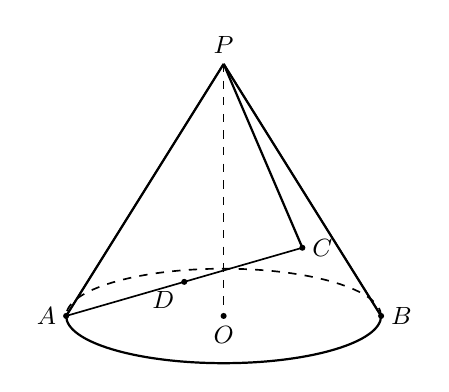
\begin{tikzpicture}[>=stealth, semithick, font=\small, scale=1.0]
  \draw[thick] (0,3.2)--(-2,0);
  \draw[thick] (0,3.2)--(2,0);
  \draw[thick] (-2,0) arc (180:360:2 and 0.6);
  \draw[dashed] (2,0) arc (0:180:2 and 0.6);
  \draw[dashed] (0,3.2)--(0,0);
  \coordinate (A) at (-2,0);
  \coordinate (B) at (2,0);
  \coordinate (C) at (1,0.866);
  \coordinate (D) at (-0.5,0.433);
  \draw[thick] (0,3.2)--(C);
  \draw (A)--(C);
  \draw (0,3.2)--(A); \draw (0,3.2)--(B);
  \fill (A) circle (1.1pt) node[left] {$A$};
  \fill (B) circle (1.1pt) node[right] {$B$};
  \fill (C) circle (1.1pt) node[right] {$C$};
  \fill (D) circle (1.1pt) node[below left] {$D$};
  \fill (0,0) circle (1.1pt) node[below] {$O$};
  \node[above] at (0,3.2) {$P$};
\end{tikzpicture}
\end{center}
\nopagebreak[4]
\end{question}
\begin{question}
\gkti{20}某企业在第 $1$ 年初购买一台价值为 $120$ 万元的设备 $M$，$M$ 的价值在使用过程中逐年减少。从第 $2$ 年到第 $6$ 年，每年初 $M$ 的价值比上年初减少 $10$ 万元；从第 $7$ 年开始，每年初 $M$ 的价值为上年初的 $75\%$。

（1） 求第 $n$ 年初 $M$ 的价值 $a_n$ 的表达式；

（2） 设 $A_n=\dfrac{a_1+a_2+\cdots+a_n}{n}$，若 $A_n$ 大于 $80$ 万元，则 $M$ 继续使用，否则须在第 $n$ 年初对 $M$ 更新。证明：须在第 $9$ 年初对 $M$ 更新。

\end{question}
\begin{question}
\gkti{21}已知平面内一动点 $P$ 到点 $F(1,0)$ 的距离与点 $P$ 到 $y$ 轴的距离的差等于 $1$。

（1） 求动点 $P$ 的轨迹 $C$ 的方程；

（2） 过点 $F$ 作两条斜率存在且互相垂直的直线 $l_1$，$l_2$，设 $l_1$ 与轨迹 $C$ 相交于点 $A$，$B$，$l_2$ 与轨迹 $C$ 相交于点 $D$，$E$，求 $\overrightarrow{AD}\cdot\overrightarrow{EB}$ 的最小值。

\end{question}
\begin{question}
\gkti{22}设函数 $f(x)=x-\dfrac1x-a\ln x$（$a\in\mathbf R$）。

（1） 讨论函数 $f(x)$ 的单调性；

（2） 若 $f(x)$ 有两个极值点 $x_1$ 和 $x_2$，记过点 $A(x_1,f(x_1))$，$B(x_2,f(x_2))$ 的直线斜率为 $k$。问：是否存在 $a$，使得 $k=2-a$？若存在，求出 $a$ 的值；若不存在，请说明理由。

\end{question}